\chapter{Experimental Results}
\label{chp:results}
We implemented the system architecture proposed in \secref{sec:architecture} in C++, using g++ 4.8.4 and the C++11
\citep{cpp11spec} features. With the system architecture in place, we then implemented the GSB data listener and the FP
data processor.

Our comparison experiments were performed in a linux box with Intel Xeon Quad processor and 14GB of main memory running
Ubuntu Server 14.04. We used four datasets (real and synthetic) in our experiments, with some of them having more than
50M entries and 2K unique $O_{id}$.

We compare BitDF running time and number of disks generated against an implementation of BFE, running in the same
machine, using the same datasets and parameter values. The metrics used for each dataset were (a) CPU time and (b)
Number of disks. In (a), for each flock parameter ($\mu$, $\delta$ and $\epsilon$) we fixed it in a specific value and
varied the others, in order to see how the algorithm behaves. For (b), we analyzed the cumulative number of disks
generated over time.

Before showing the results, there are some analysis outcomes that will hold for any dataset analyzed here:

\begin{enumerate}
    \item \textbf{$\delta$ variation}: The longer the flock patterns we try to find (long $\delta$), the more disks will
        stay cached being analyzed and trying to be merged with new disks from time slots to come. This can have a big
        impact in running time.\label{sssec:lvariation}

    \item \textbf{$\epsilon$ variation}: As the disk radius ($\epsilon$) gets bigger, more points will be clustered
        inside a disk and thus more intersections and duplicates of those disks as more likely to be founf. This will
        affect the time spent in analyzing disks from one time slot to another. \label{sssec:gvariation}

    \item \textbf{$\mu$ variation}: By increasing $\mu$, it gets more and more difficult to find disks that are flock
        candidates ($|D| \ge \mu$), so less disks are generated. This scenario is where BitDF will achieve less
        improvements. \label{sssec:nvariation}
\end{enumerate}

\section{Trucks Dataset}
\label{subsec:trucks}
This was one of the datasets that Vieira et al. \citep{vieira} used in the experiments of BFE, but the authors modified
such dataset \citep{trucksdataset}, resulting in a data set which is way far from those found in real world analysis. In
their modification, every time interval is of one second, the GPS coordinates were mapped to a $\mathbb{R}^2$ coordinate
system (ranging from 0 to 1000) and most of the points are present in each time interval. The modified dataset resulted
in 112203 entries and 276 unique $O_{id}$ (instead of 50 in the original dataset).

\begin{figure*}[h!]
    \centering
    \begin{subfigure}[t]{0.48\textwidth}
        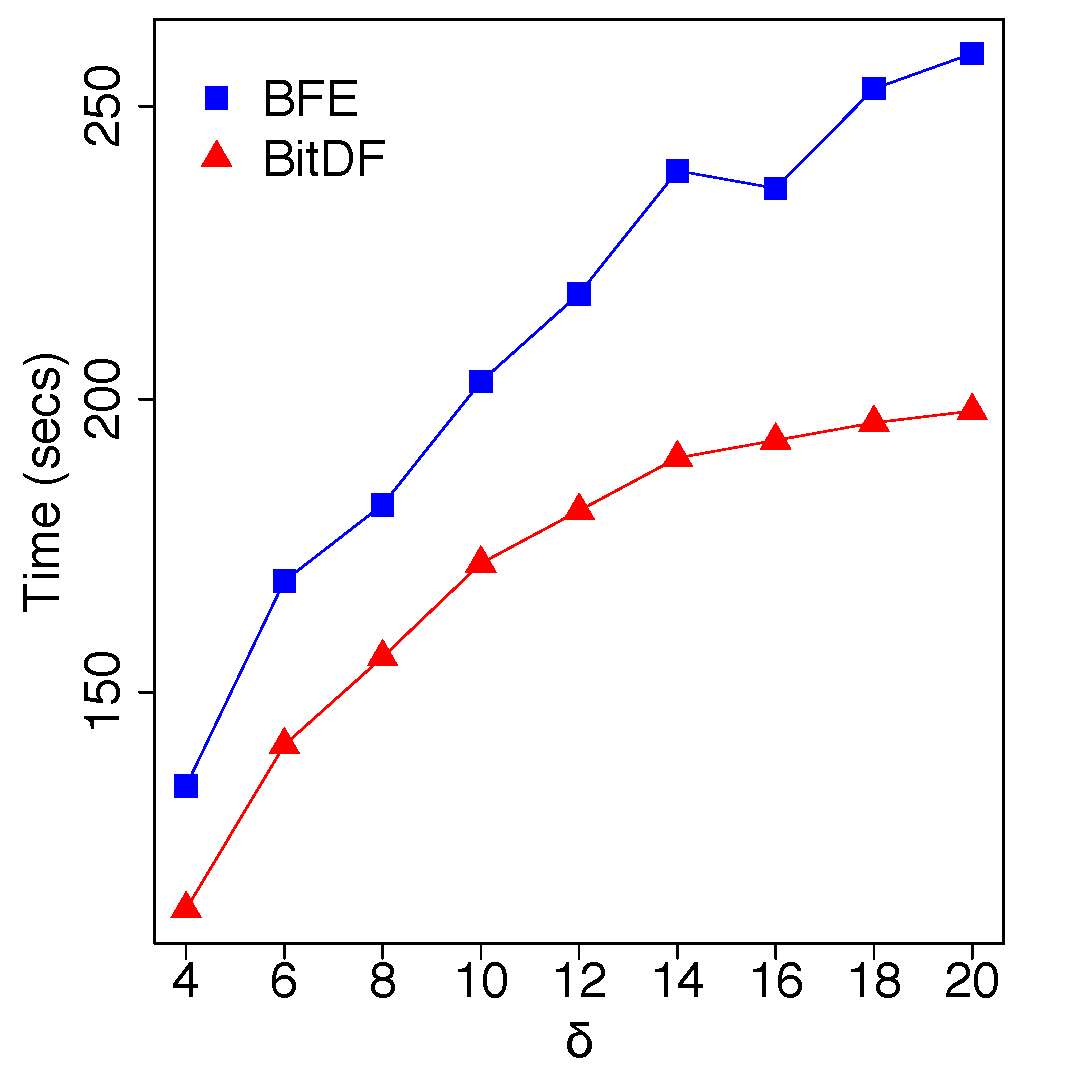
\includegraphics[width=\textwidth]{images/Trucks_n_4_g_1_5_varying_l.eps}
        \caption{$\mu = 4$, $\epsilon = 1.5$ and $\delta$ varying}
        \label{fig:trucks_vary_l}
    \end{subfigure}
    \begin{subfigure}[t]{0.48\textwidth}
        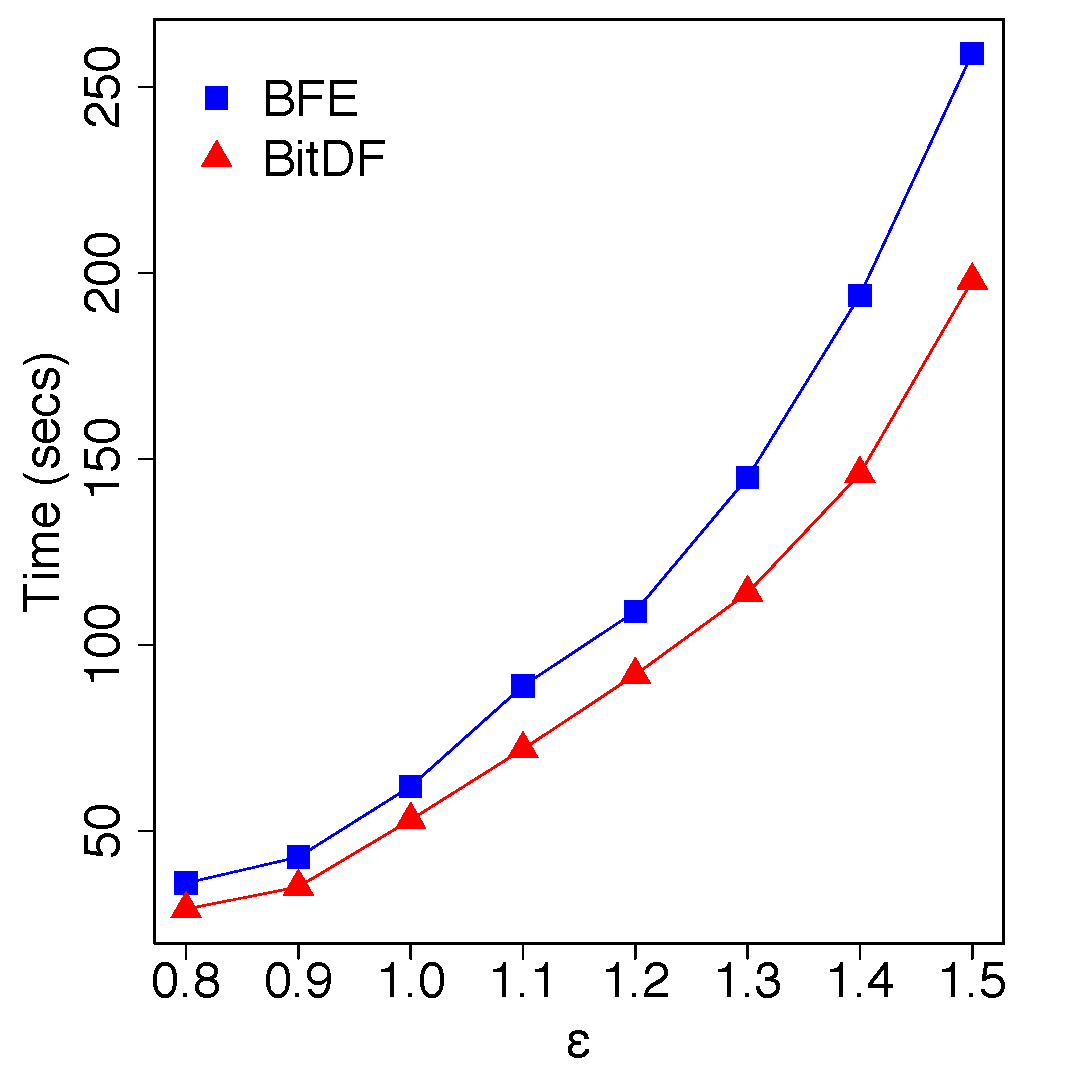
\includegraphics[width=\textwidth]{images/Trucks_n_4_l_20_varying_g.eps}
        \caption{$\mu = 4$, $\delta = 20$ and $\epsilon$ varying}
        \label{fig:trucks_vary_g}
    \end{subfigure}
    \caption{Results varying $\delta$ and $\epsilon$ for Trucks dataset}
    \label{fig:trucks_results}
\end{figure*}

\begin{figure*}[h!]
    \begin{subfigure}[t]{0.48\textwidth}
        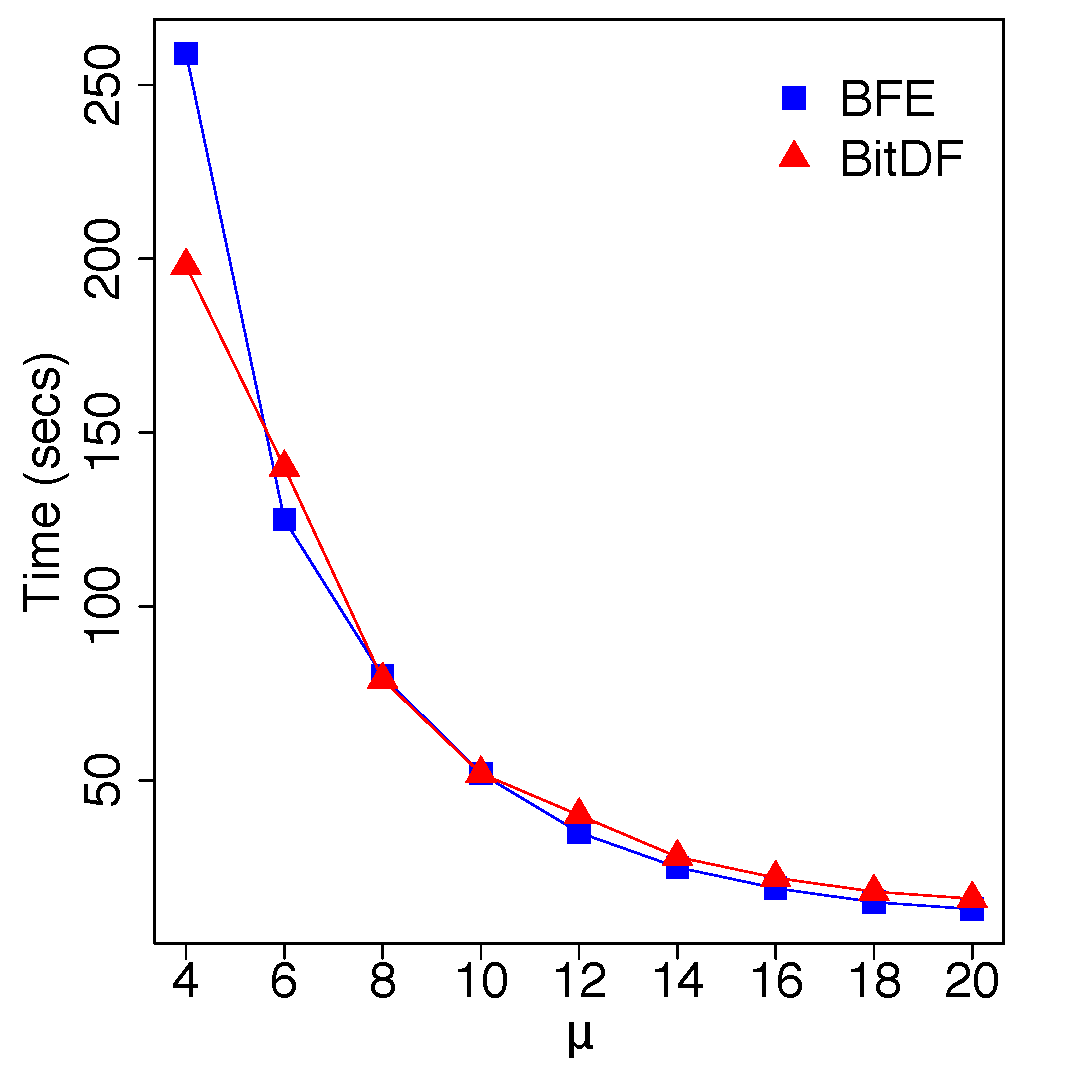
\includegraphics[width=\textwidth]{images/Trucks_l_20_g_1_5_varying_n.eps}
        \caption{$\delta = 20$, $\epsilon = 1.5$ and $\mu$ varying}
        \label{fig:trucks_vary_n}
    \end{subfigure}
    \begin{subfigure}[t]{0.48\textwidth}
        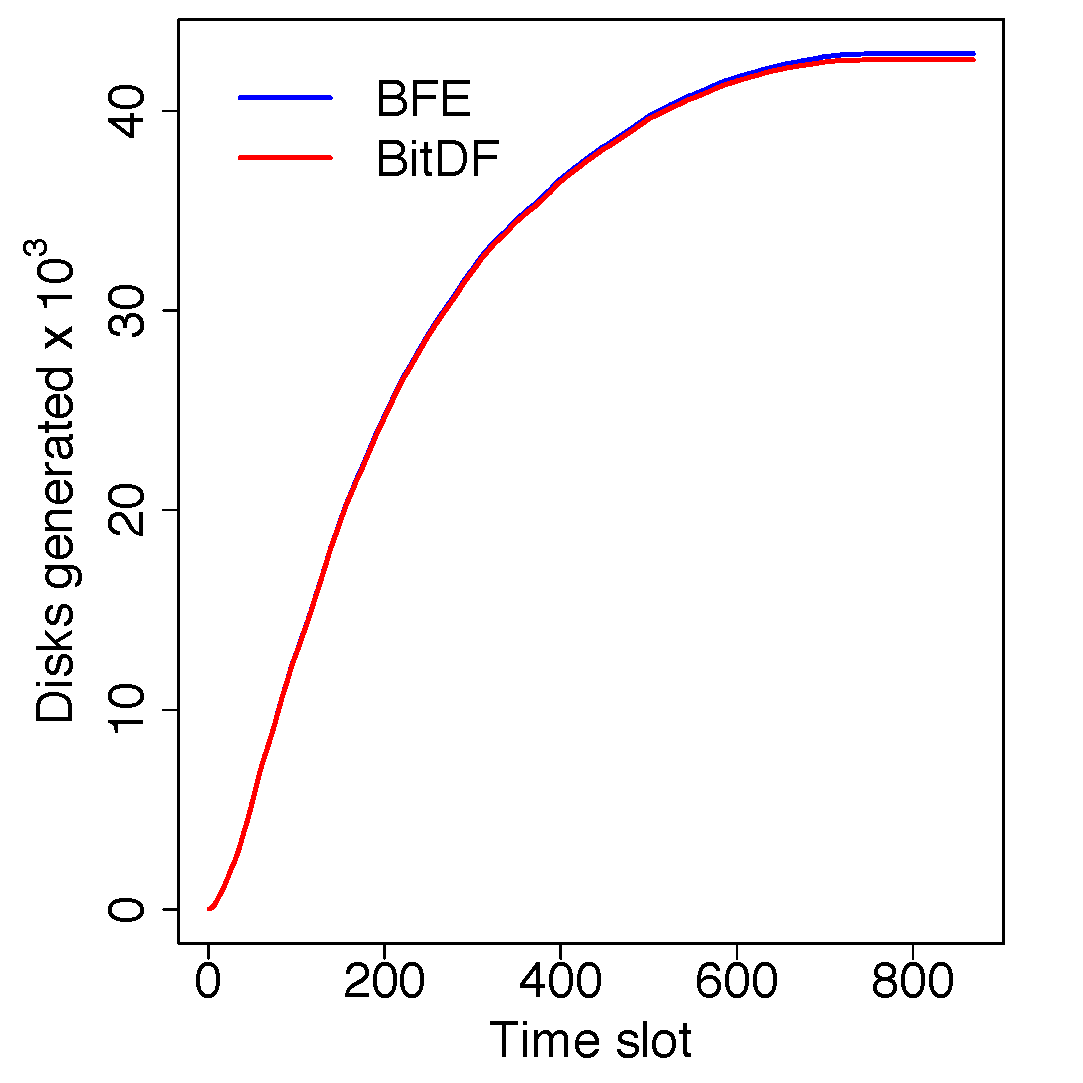
\includegraphics[width=\textwidth]{images/Trucks_d.eps}
        \caption{Cumulative disks by time}
        \label{fig:trucks_disks}
    \end{subfigure}
    \caption{Results varying $\mu$ and number of disks generated over time for Trucks dataset}
    \label{fig:trucks_results2}
\end{figure*}

By looking at \figref{fig:trucks_results} and \figref{fig:trucks_results2}, we can see that we have some gains in
execution time. However, they are not too significant due to the fact that the number of disks generated by each time
slot does not differ too much between BFE and BitDF, as we can see in \figref{fig:trucks_disks}. This happens because
almost all points appear in every single time slot, then buffering and mapping the $O_{id}$ presence in time does not
make a big impact, since we will not be able to filter out disks created with points not being present in $\delta$
consecutive time slots.  \figref{fig:trucks_vary_l} and \figref{fig:trucks_vary_g} show some running time improvements
against BFE, which are backed up by the explanations given at~\ref{sssec:lvariation} and~\ref{sssec:gvariation}. A
different behavior is observed in \figref{fig:trucks_vary_n}, in which BitDF starts better but ends up almost tied with
BFE, which can be explained by~\ref{sssec:nvariation}, but is also very influenced by the dataset modifications.

\section{BerlinMOD Dataset}
\label{subsec:berlinmod}
BerlinMOD consists in a traffic generation model \citep{berlinmodpaper} used to create sythentic datasets of moving
objects. This particular dataset that we are analysing was the biggest one that we could find in the set of synthetic
datasets that are available in their website \citep{berlinmod} and consists of 56,127,943 entries and 2000 unique
$O_{id}$.

\begin{figure*}[h!]
    \centering
    \begin{subfigure}[t]{0.48\textwidth}
        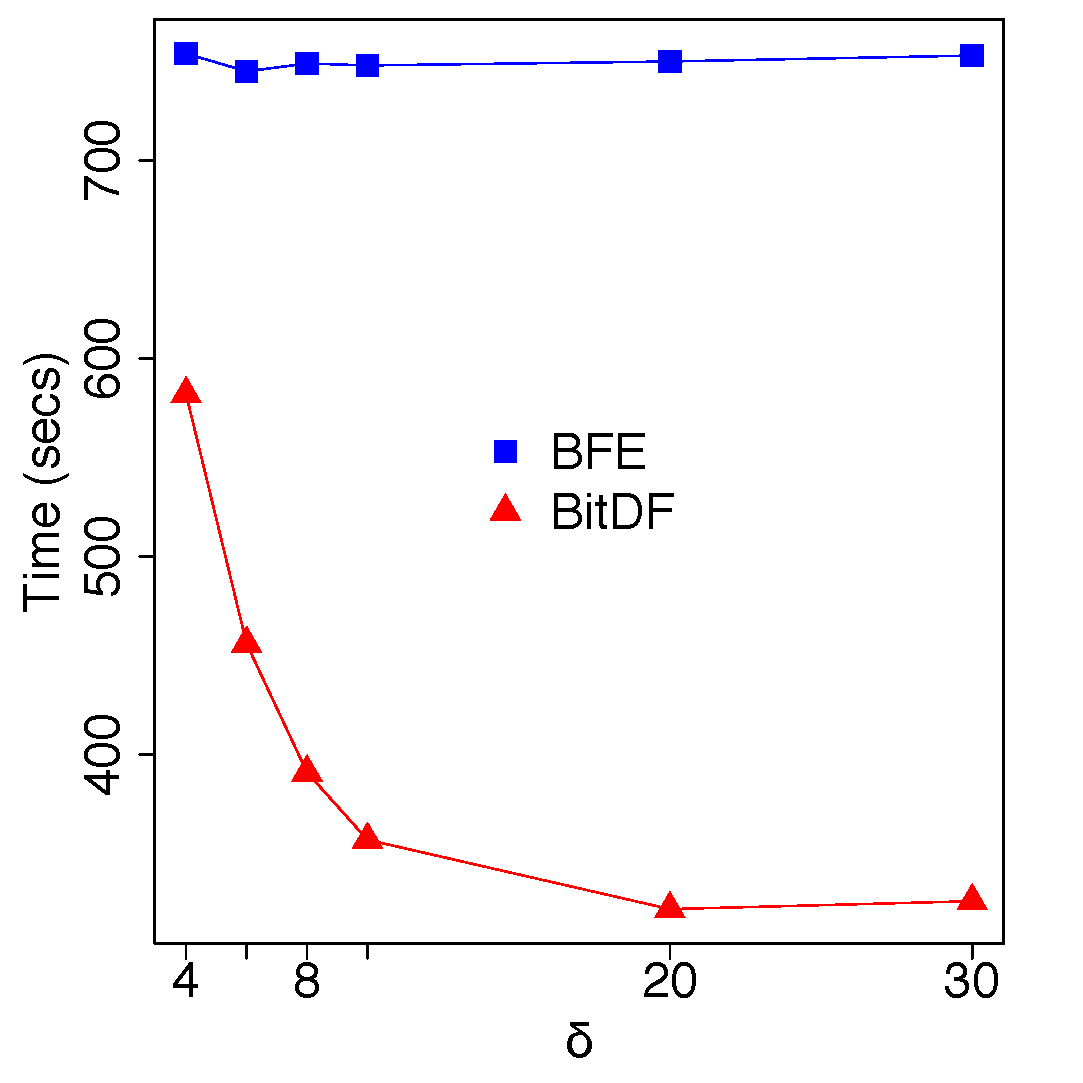
\includegraphics[width=\textwidth]{images/BerlinMOD_n_4_g_100_varying_l.eps}
        \caption{$\mu = 4$, $\epsilon = 100$ and $\delta$ varying}
        \label{fig:berlinmod_vary_l}
    \end{subfigure}
    \begin{subfigure}[t]{0.48\textwidth}
        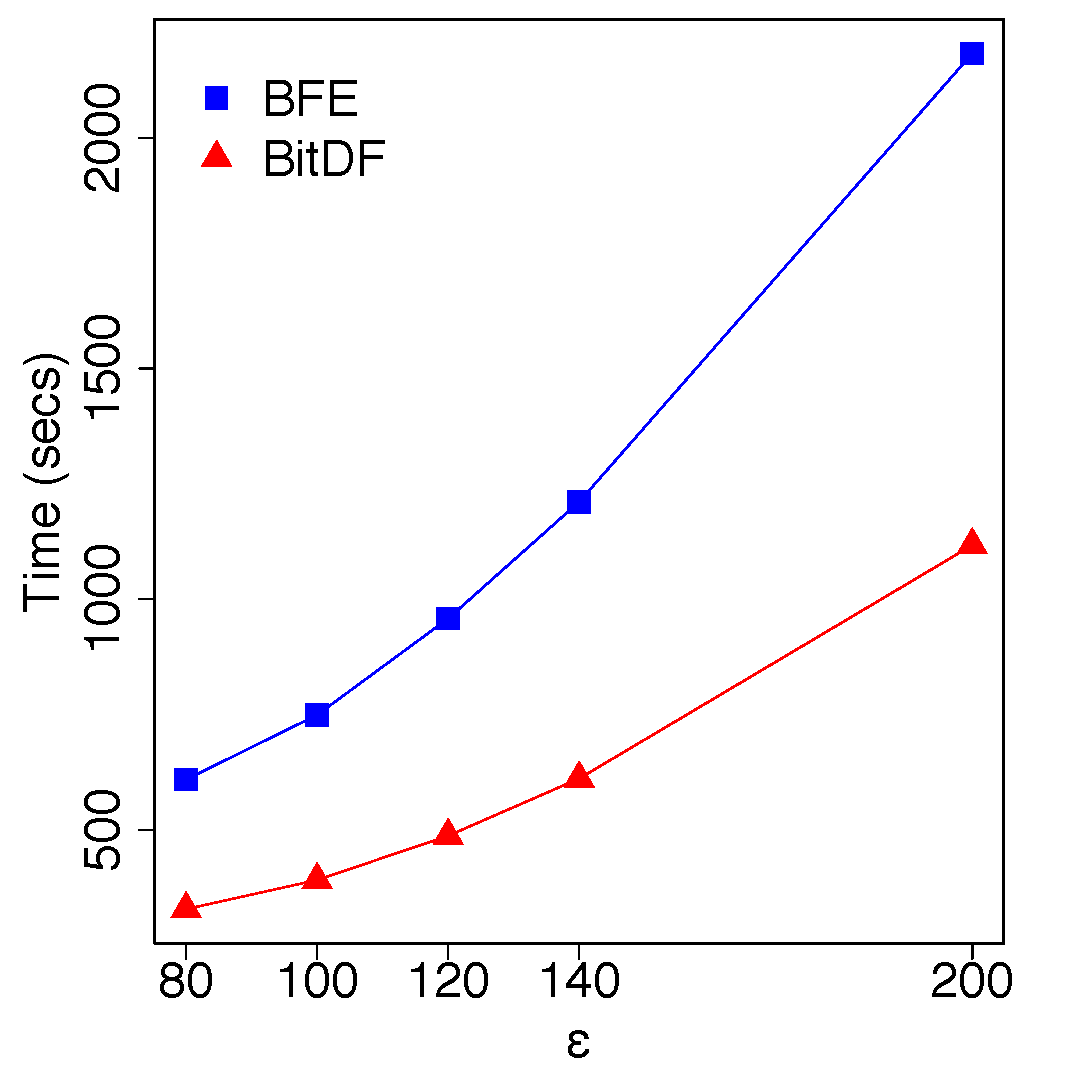
\includegraphics[width=\textwidth]{images/BerlinMOD_n_4_l_8_varying_g.eps}
        \caption{$\mu = 4$, $\delta = 8$ and $\epsilon$ varying}
        \label{fig:berlinmod_vary_g}
    \end{subfigure}
    \caption{Results varying $\delta$ and $\epsilon$ for BerlinMOD dataset}
    \label{fig:berlinmod_results}
\end{figure*}

\begin{figure*}[h!]
    \begin{subfigure}[t]{0.48\textwidth}
        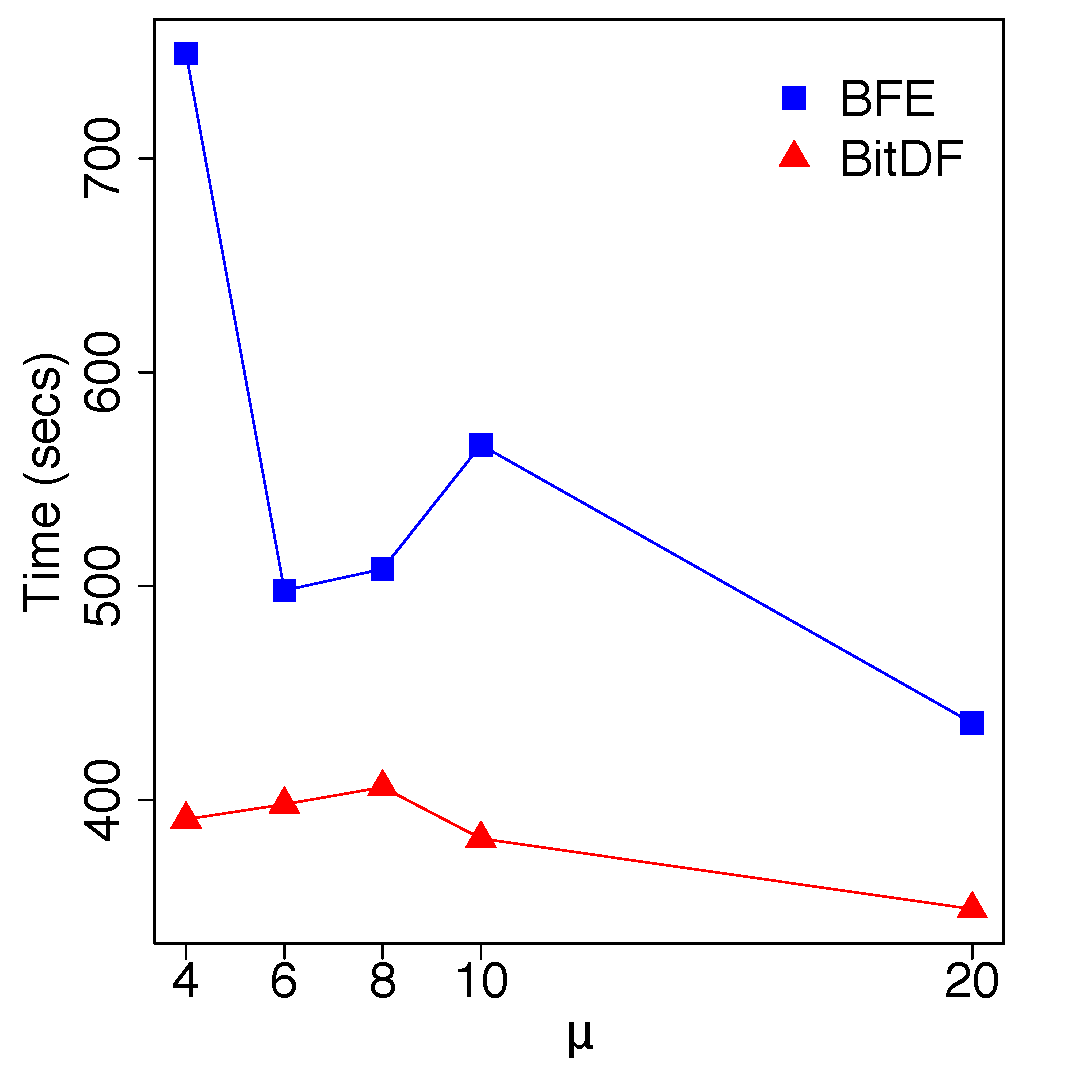
\includegraphics[width=\textwidth]{images/BerlinMOD_l_8_g_100_varying_n.eps}
        \caption{$\delta = 8$, $\epsilon = 100$ and $\mu$ varying}
        \label{fig:berlinmod_vary_n}
    \end{subfigure}
    \begin{subfigure}[t]{0.48\textwidth}
        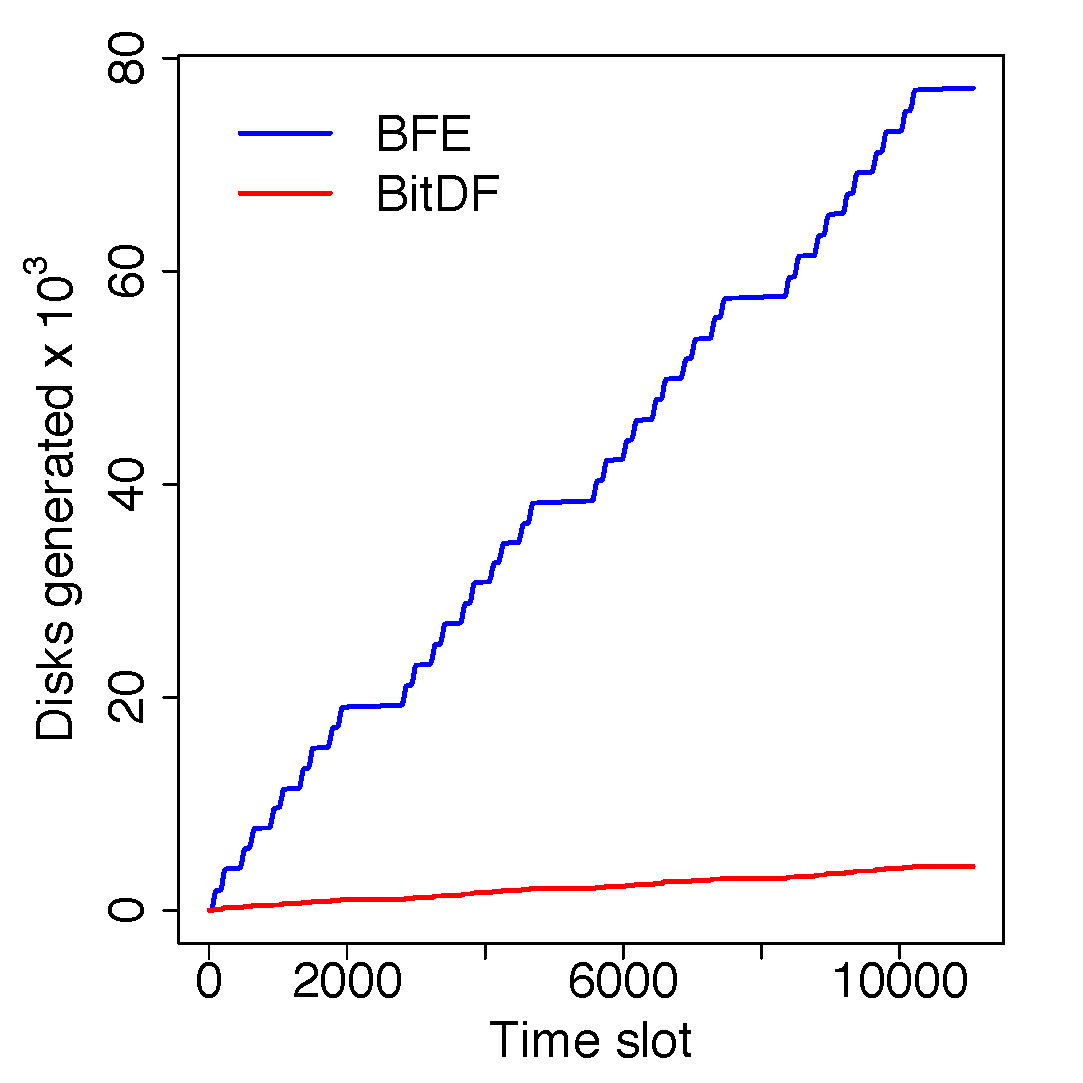
\includegraphics[width=\textwidth]{images/BerlinMOD_d.eps}
        \caption{Cumulative disks by time}
        \label{fig:berlinmod_disks}
    \end{subfigure}
    \caption{Results varying $\mu$ and number of disks generated over time for BerlinMOD dataset}
    \label{fig:berlinmod_results2}
\end{figure*}

As we can see by the results presented in \figref{fig:berlinmod_results} and \figref{fig:berlinmod_results2}, BitDF was
able to achieve great performance gains over BFE, in some cases being 57\% faster (\figref{fig:berlinmod_vary_l}). In
\figref{fig:berlinmod_disks} it is shown that BitDF reduces the cumulative number of disks created over time in 94\%, by
only creating disks that can indeed form flock patterns, which justifies the great improvements that BitDF was able to
get in this dataset.  Differently from the results presented in~\ref{subsec:trucks}, even with a growing $\mu$, BitDF
was able to get great improvements over BFE, ranging from 20\% to 48\%, as depicted in \figref{fig:berlinmod_vary_n}. It
is also worth mentioning the gain in running time that BitDF was able to achieve when we varied the $\epsilon$
parameter, reaching 48\%, as shown in \figref{fig:berlinmod_vary_g}

\section{TDrive Dataset}
\label{subsec:tdrive}
This is a real dataset, having spatio-temporal data describing one week of taxis' trajectories of taxis in Beijing,
China, available in \citep{tdrive}. It has 17,762,489 entries with 10336 unique $O_{id}$.

\begin{figure*}[h!]
    \centering
    \begin{subfigure}[t]{0.48\textwidth}
        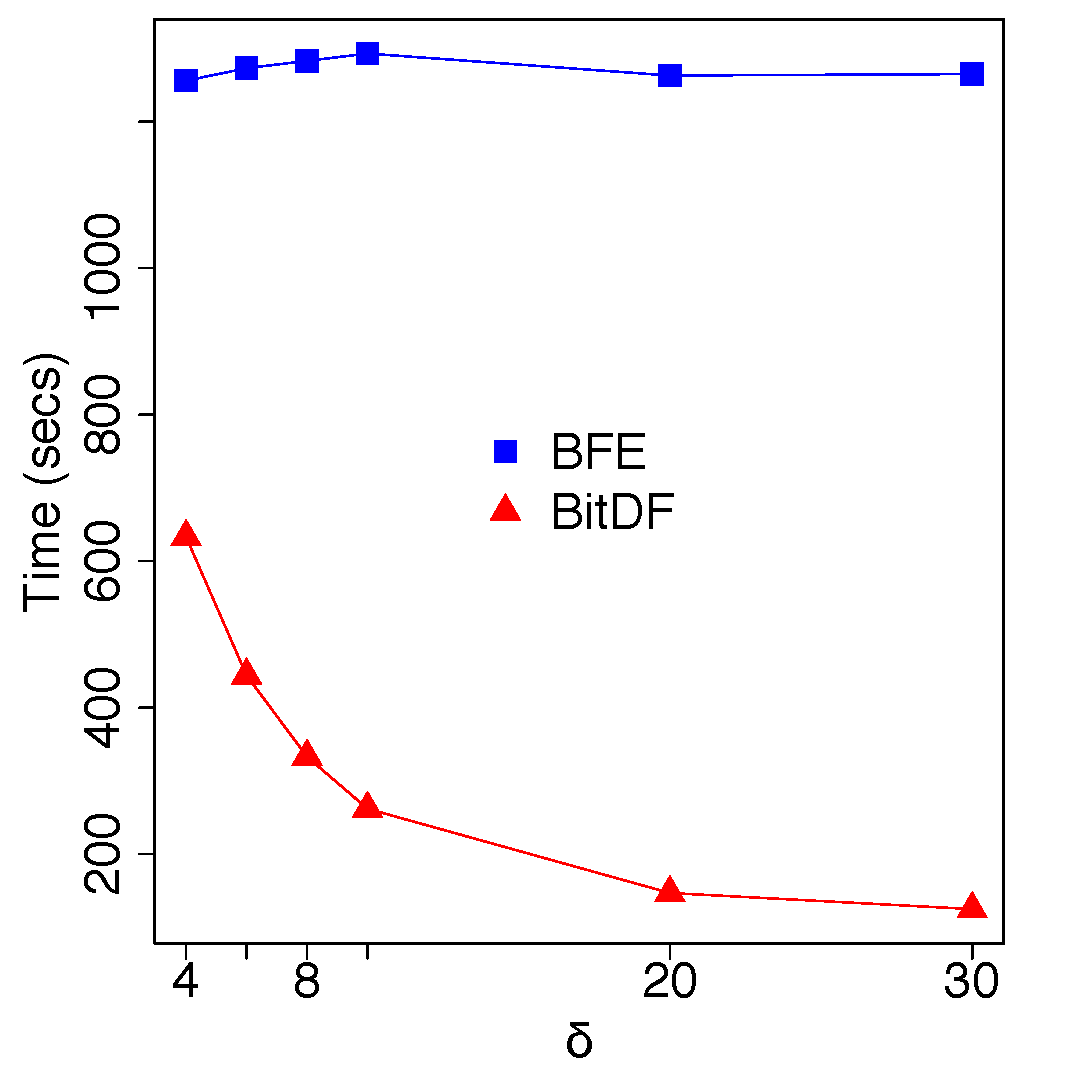
\includegraphics[width=\textwidth]{images/TDrive_n_4_g_100_varying_l.eps}
        \caption{$\mu = 4$, $\epsilon = 100$ and $\delta$ varying}
        \label{fig:tdrive_vary_l}
    \end{subfigure}
    \begin{subfigure}[t]{0.48\textwidth}
        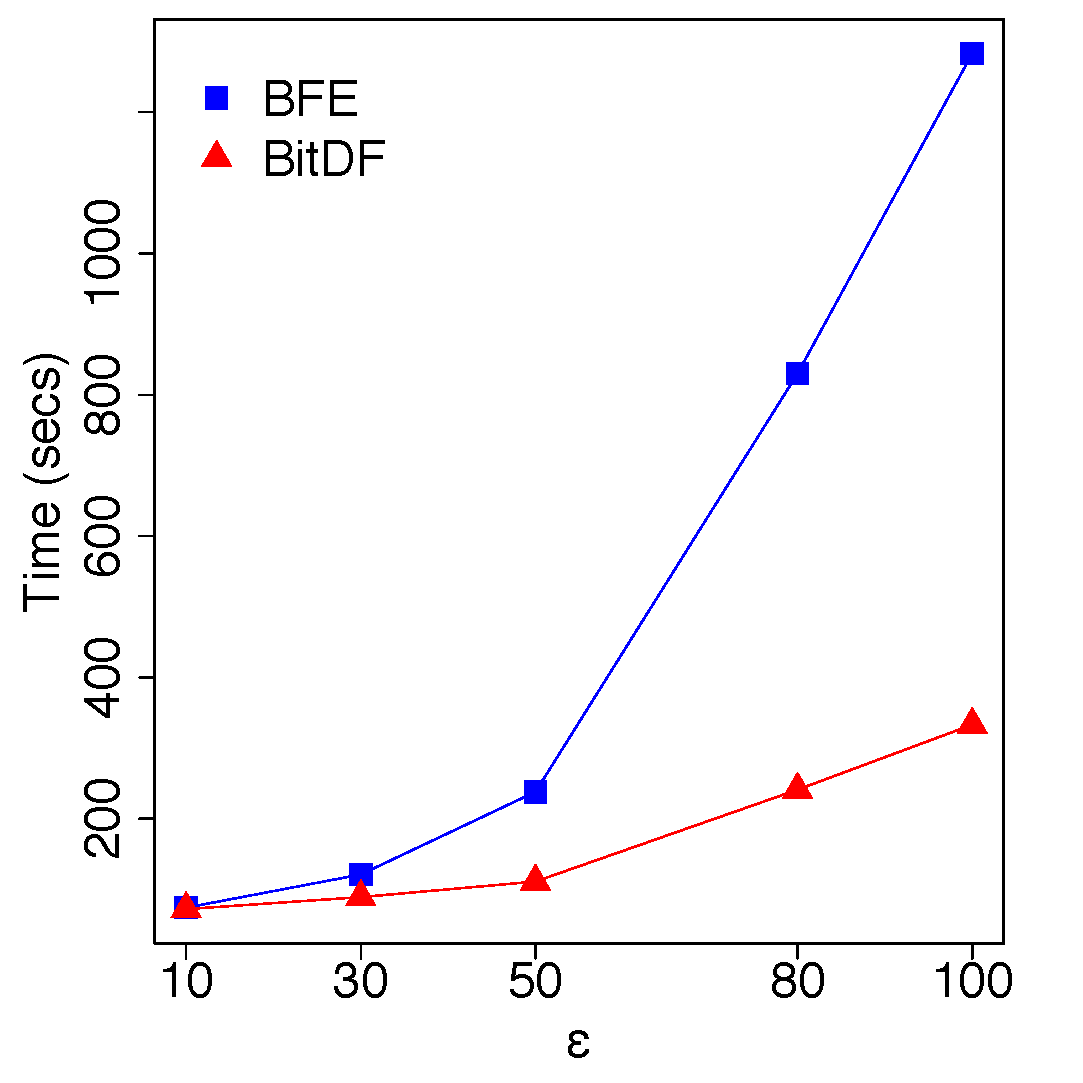
\includegraphics[width=\textwidth]{images/TDrive_n_4_l_8_varying_g.eps}
        \caption{$\mu = 4$, $\delta = 8$ and $\epsilon$ varying}
        \label{fig:tdrive_vary_g}
    \end{subfigure}
    \caption{Results varying $\delta$ and $\epsilon$ for TDrive dataset}
    \label{fig:tdrive_results}
\end{figure*}

One can see by the results presented in \figref{fig:tdrive_results} and \figref{fig:tdrive_results2}, that BitDF was
able to dramatically reduce the execution time, when compared to BFE. When varying the $\delta$ parameter, the running
time improvement was of almost 90\%, droping from 1,2265 seconds to only 125 seconds of processing time, as shown in
\figref{fig:tdrive_vary_l}. Continuing the improvements, in \figref{fig:tdrive_vary_g} we can see that BitDF reduced the
execution time up to 74\% when varying $\epsilon$. Additionally, despite seeing some similar behavior with the other
analyzed datasets (like presented in \secref{subsec:trucks}) when varying $\mu$, \figref{fig:tdrive_vary_n} shows that
BitDF was able to improve the execution time by 74\% in some cases. It is also worth noting that the results achieved
are a reflex of the huge decrease of disks that were generated by time, as depicted in \figref{fig:tdrive_disks},
reaching almost 96\% of reduction.

\begin{figure*}[h!]
    \begin{subfigure}[t]{0.48\textwidth}
        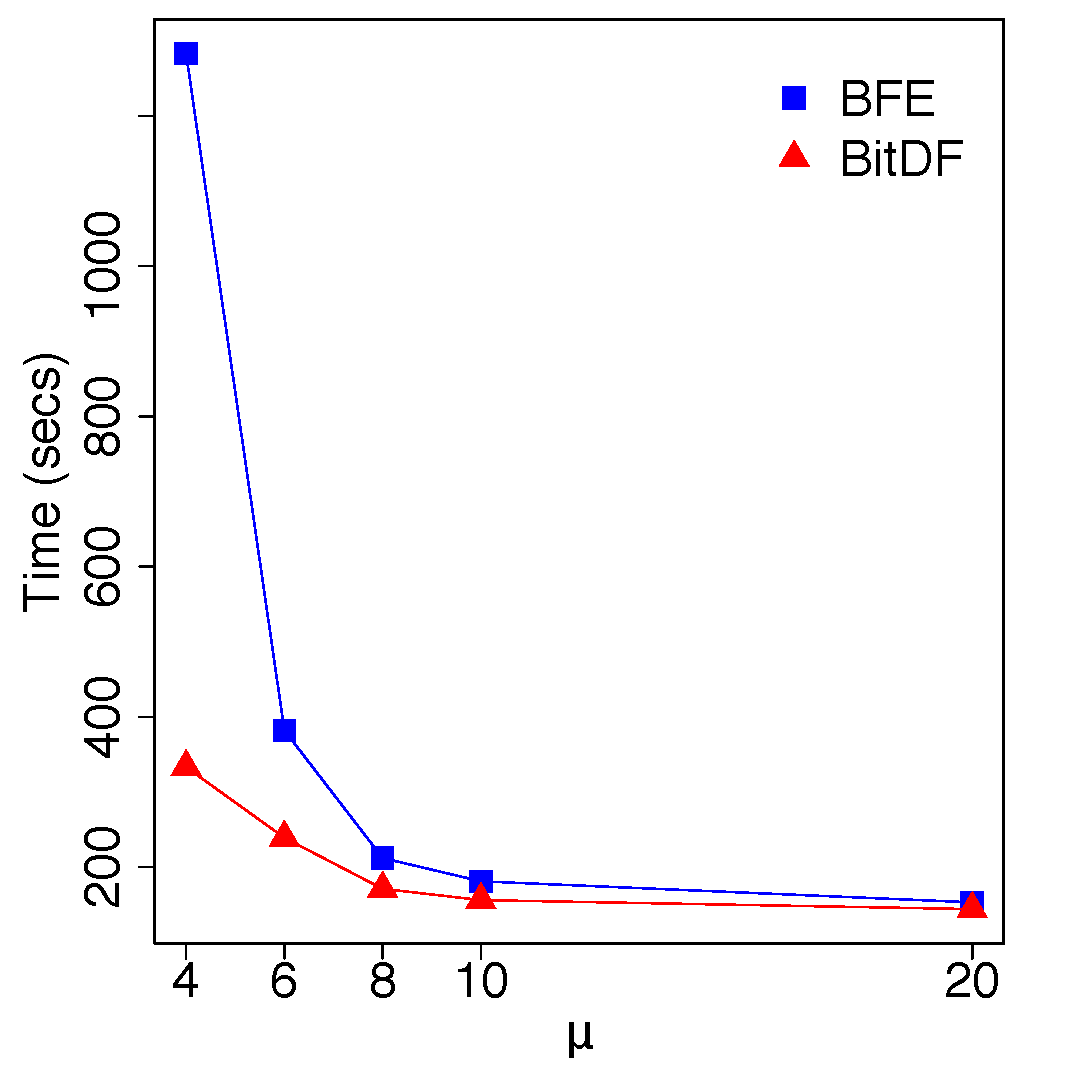
\includegraphics[width=\textwidth]{images/TDrive_l_8_g_100_varying_n.eps}
        \caption{$\delta = 8$, $\epsilon = 100$ and $\mu$ varying}
        \label{fig:tdrive_vary_n}
    \end{subfigure}
    \begin{subfigure}[t]{0.48\textwidth}
        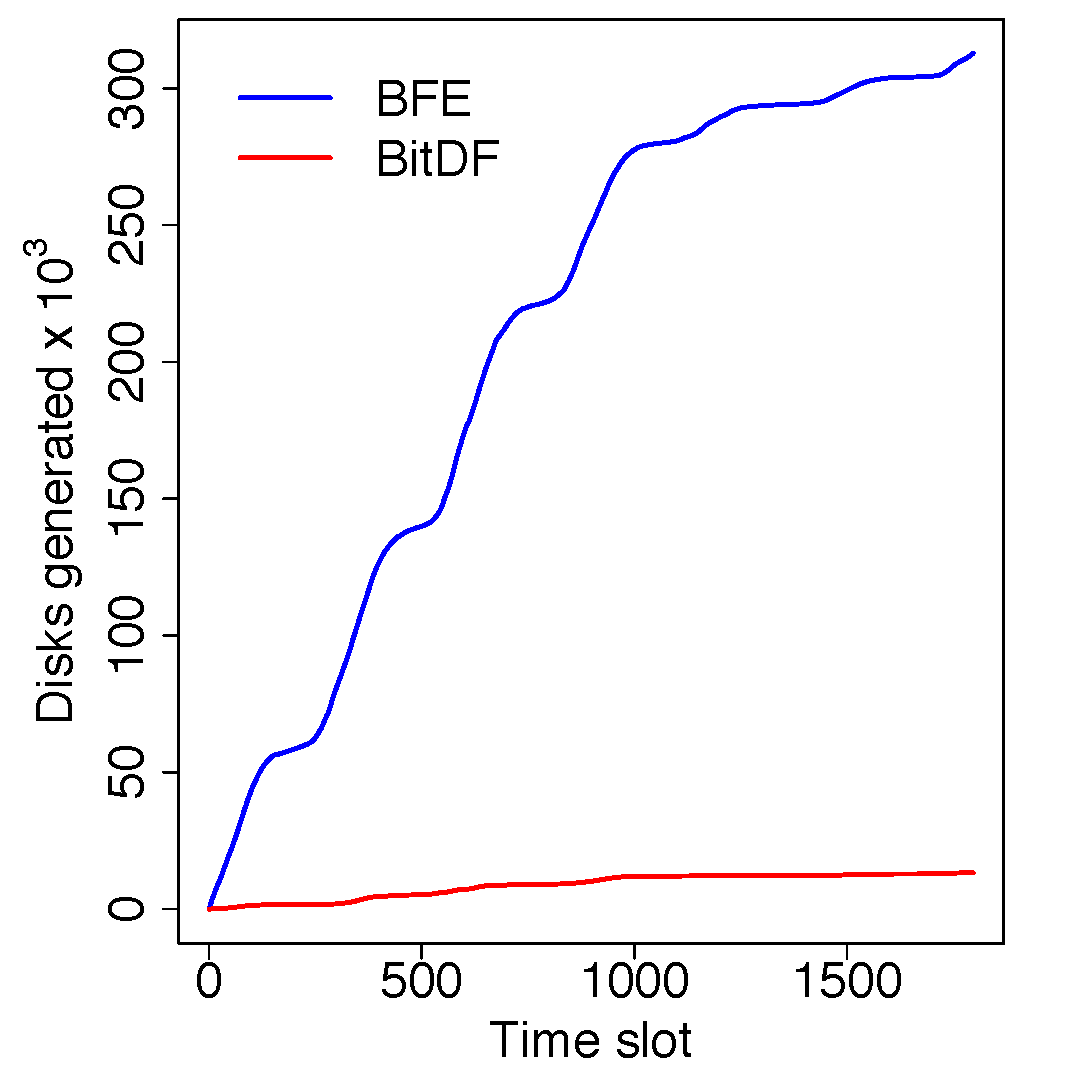
\includegraphics[width=\textwidth]{images/TDrive_d.eps}
        \caption{Cumulative disks by time}
        \label{fig:tdrive_disks}
    \end{subfigure}
    \caption{Results varying $\mu$ and number of disks generated over time for TDrive dataset}
    \label{fig:tdrive_results2}
\end{figure*}

\section{Brinkkhoff Dataset}
\label{subsec:brinkhoff}
Likewise BerlinMOD, Brinkhoff is also a city traffic generation model \citep{brinkhoffpaper}. We generated a synthetic
dataset using the Minnesota Web-based Traffic Generator \citep{mntg}, having 2000 as the "Starting Vehicles" and 100 as
the "Simulation Time" parameters, which are the largest allowed numbers for them. The result dataset has 314,523 entries
and 7000 unique $O_{id}$.

\begin{figure*}[h!]
    \centering
    \begin{subfigure}[t]{0.48\textwidth}
        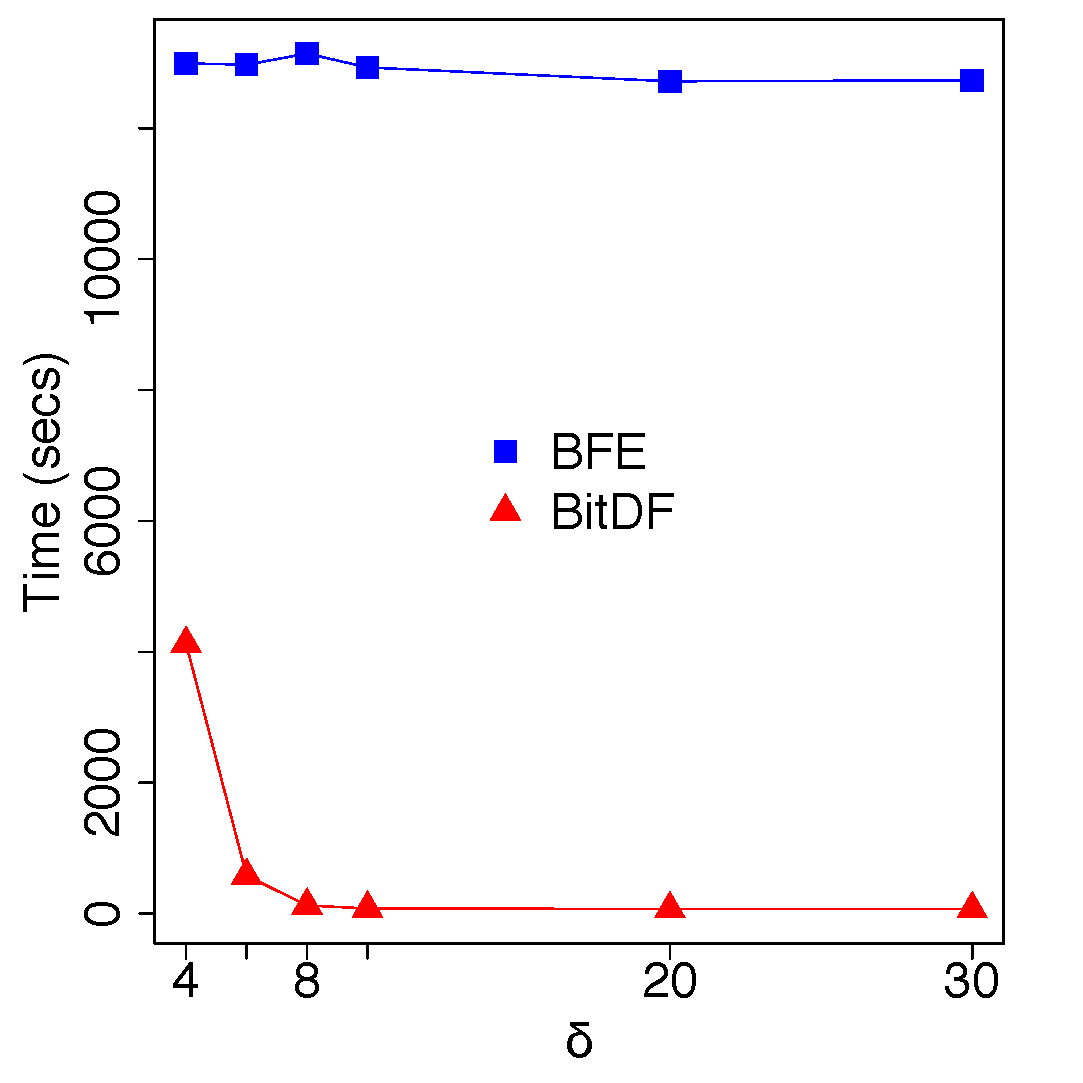
\includegraphics[width=\textwidth]{images/Brinkhoff_n_4_g_200_varying_l.eps}
        \caption{$\mu = 4$, $\epsilon = 200$ and $\delta$ varying}
        \label{fig:brinkhoff_vary_l}
    \end{subfigure}
    \begin{subfigure}[t]{0.48\textwidth}
        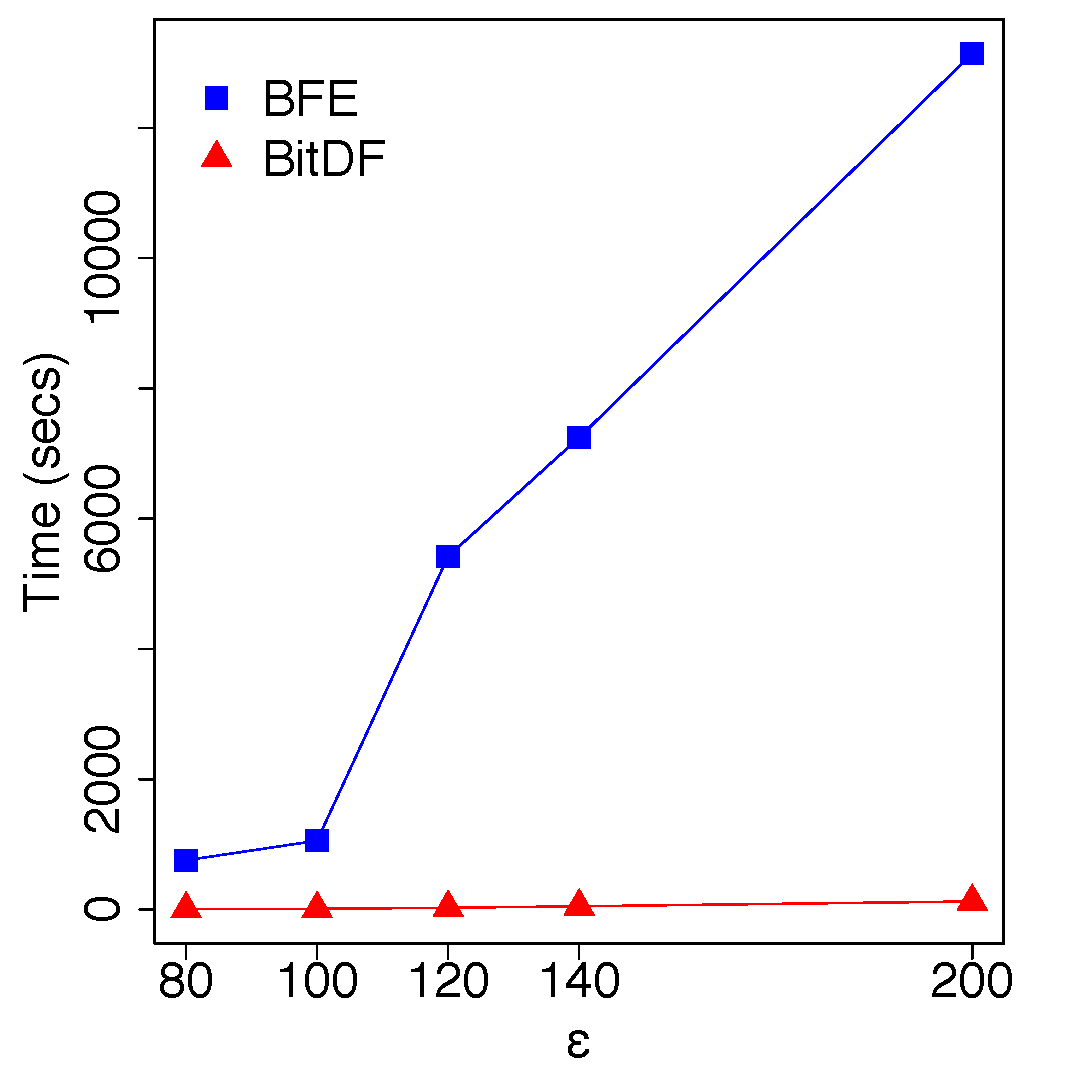
\includegraphics[width=\textwidth]{images/Brinkhoff_n_4_l_8_varying_g.eps}
        \caption{$\mu = 4$, $\delta = 8$ and $\epsilon$ varying}
        \label{fig:brinkhoff_vary_g}
    \end{subfigure}
    \caption{Results varying $\delta$ and $\epsilon$ for Brinkhoff dataset}
    \label{fig:brinkhoff_results}
\end{figure*}

\begin{figure*}[h!]
    \begin{subfigure}[t]{0.48\textwidth}
        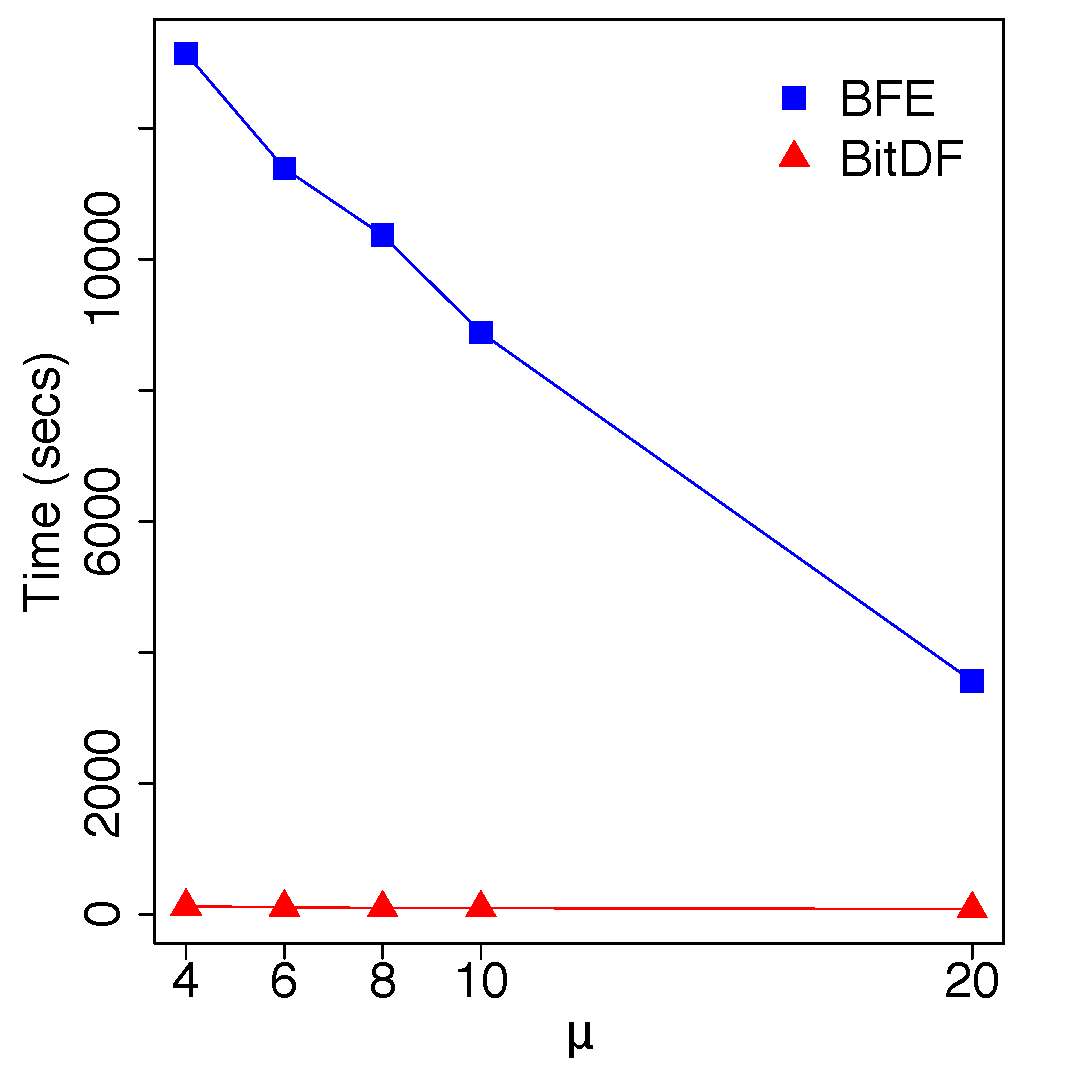
\includegraphics[width=\textwidth]{images/Brinkhoff_l_8_g_200_varying_n.eps}
        \caption{$\delta = 8$, $\epsilon = 200$ and $\mu$ varying}
        \label{fig:brinkhoff_vary_n}
    \end{subfigure}
    \begin{subfigure}[t]{0.48\textwidth}
        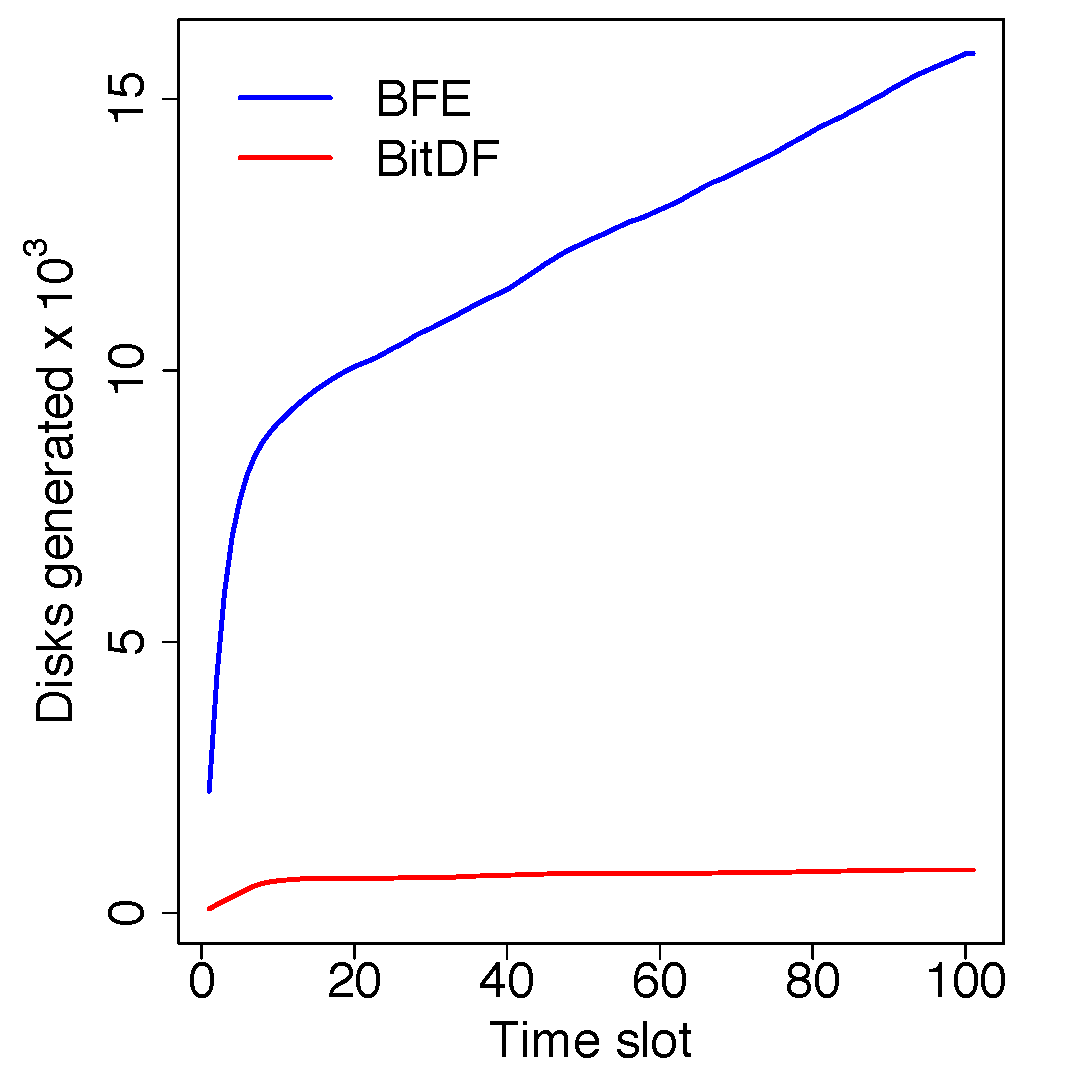
\includegraphics[width=\textwidth]{images/Brinkhoff_d.eps}
        \caption{Cumulative disks by time}
        \label{fig:brinkhoff_disks}
    \end{subfigure}
    \caption{Results varying $\mu$ and number of disks generated over time for Brinkhoff dataset}
    \label{fig:brinkhoff_results2}
\end{figure*}

The results achieved with this dataset were the best that BitDF was able to get amongst the other datasets analyzed in
this thesis, as one can notice by looking to \figref{fig:brinkhoff_results} and \figref{fig:brinkhoff_results2}. There
were huge drops in execution time, as depicted in \figref{fig:brinkhoff_vary_l}, where BitDF analyzed the whole dataset
in only 69 seconds, while BFE took 12,732 seconds, representing an improvement of 99.5\%. Another great running time
improvement of 99\% can be seen when we varied the $\epsilon$ parameter, as shown in \figref{fig:brinkhoff_vary_g},
droping from 13,141 seconds to 125 seconds. We can see in \figref{fig:brinkhoff_vary_n} that even with the variation of
$\mu$, BitDF was able to show huge improvement, with results ranging from 98\% to 99\% of CPU time reduction.
Additionally, we can see in \figref{fig:brinkhoff_disks} that we were able to reduce the number of disks by 95\%, what
is a huge improvement and is reflecting directly in the running time improvements that we could see with this dataset.
